%%%%%%%%%%%%%%%%%%%%%%%%%%%%%%%%%%%%%%%%%%%
%%% DOCUMENT PREAMBLE %%%
\documentclass[12pt]{report}
\usepackage[english]{babel}
%\usepackage{natbib}
\usepackage{url}
\usepackage[utf8x]{inputenc}
\usepackage{amsmath}
\usepackage{graphicx}
\graphicspath{{images/}}
\usepackage{parskip}
\usepackage{fancyhdr}
\usepackage{vmargin}
\usepackage{listings}
\usepackage{protobuf/lang}  % include language definition for protobuf
\usepackage{protobuf/style}
\usepackage{graphicx}
\usepackage{caption}
\setmarginsrb{3 cm}{2.5 cm}{3 cm}{2.5 cm}{1 cm}{1.5 cm}{1 cm}{1.5 cm}

\title{1}								
% Title
\author{Joel Klimont}						
% Author
\date{10.3.2019}
% Date

\makeatletter
\let\thetitle\@title
\let\theauthor\@author
\let\thedate\@date
\makeatother

\pagestyle{fancy}
\fancyhf{}
\rhead{\theauthor}
\lhead{\thetitle}
\cfoot{\thepage}
%%%%%%%%%%%%%%%%%%%%%%%%%%%%%%%%%%%%%%%%%%%%
\begin{document}

%%%%%%%%%%%%%%%%%%%%%%%%%%%%%%%%%%%%%%%%%%%%%%%%%%%%%%%%%%%%%%%%%%%%%%%%%%%%%%%%%%%%%%%%%

\begin{titlepage}
	\centering
    \vspace*{0.5 cm}
   % \includegraphics[scale = 0.075]{bsulogo.png}\\[1.0 cm]	% University Logo
\begin{center}    \textsc{\Large   NVS Project 5th Class}\\[2.0 cm]	\end{center}% University Name
	\textsc{\Large Robocode}\\[0.5 cm]				% Course Code
	\rule{\linewidth}{0.2 mm} \\[0.4 cm]
	{ \huge \bfseries \thetitle}\\
	\rule{\linewidth}{0.2 mm} \\[1.5 cm]
	
	\begin{minipage}{0.4\textwidth}
		\begin{flushleft} \large
		%	\emph{Submitted To:}\\
		%	Name\\
          % Affiliation\\
           %contact info\\
			\end{flushleft}
			\end{minipage}~
			\begin{minipage}{0.4\textwidth}
            
			\begin{flushright} \large
			\emph{Submitted By :} \\
			Joel Klimont
		\end{flushright}
           
	\end{minipage}\\[2 cm]
	
	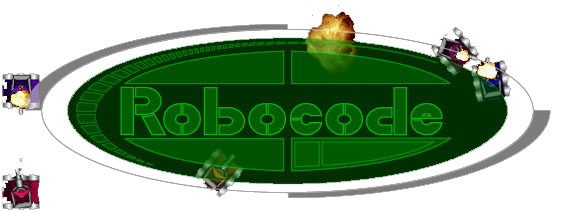
\includegraphics[scale = 0.5]{robocode_logo.jpg}
    
    
    
    
	
\end{titlepage}

%%%%%%%%%%%%%%%%%%%%%%%%%%%%%%%%%%%%%%%%%%%%%%%%%%%%%%%%%%%%%%%%%%%%%%%%%%%%%%%%%%%%%%%%%

\tableofcontents
\pagebreak

%%%%%%%%%%%%%%%%%%%%%%%%%%%%%%%%%%%%%%%%%%%%%%%%%%%%%%%%%%%%%%%%%%%%%%%%%%%%%%%%%%%%%%%%%
\renewcommand{\thesection}{\arabic{section}}
\section{Introduction}
 
\subsection{Robocode}

Robocode is a multiplayer game in which players don't directly compete against their opponents but instead they have to program a robot which fights for them. The goal is to program a robot that can defeat all opponents and survive until the end of the game.

\subsubsection{Robots}
Each robot has a starting energy of 100\%. In order to shoot a bullet at an enemy the robot has a gun that can be rotated 360° degrees. The gun also acts as a scanner. If a robot intersects with the range of the gun the program of the player will receive the position and energy of the scanned robot. What the player chooses to do with that information is completely up to him. He could for example, shoot at the player or store his position in a vector and try to predict his speed/ position using the last points as reference.

\section{Technologies}

\subsection{Asio}

Asio is a Boost C++ library that enables a developer to send and receive messages over the network. The library is open source and was accepted into the Boost library on 30 December 2005.

\subsection{Google protobuf and grpc}

\subsubsection{Protocol Buffers}

Protobuf is a language neutral way of defining messages that can be sent over the network. The following code is an example from the project:

\lstinputlisting[language=protobuf3,style=protobuf]{code_listings/example.proto}
\captionof{lstlisting}{Protobuf example}

There are two different messages defined here. The first one is a position which has two attributes an ''y'' and a ''x'' coordinate. The second message uses the first one and has two more additional attributes. The ''id'' is a unique identifier given to every robot a the start of the game. The ''energy\_left'' value describes the energy of the transmitted robot.

\subsubsection{gRPC}

GRPC stand for ''Google remote procedure calls''. It enables developers to send and receive protobuf messages over the network.

\subsection{Clipp}

Clipp is used for parsing all command line arguments from the user.

\subsection{Json}

The program can also be configured using the ''config.json'' file.

\begin{lstlisting}[frame=single]
{
  "port" : 5000,
  "streaming_port": 5010,
  "username" : "",
  "server_ip" : "",
  "background_robot": true,
  "no_menu_host": false,
  "log_level": "info"
}
\end{lstlisting}
\captionof{lstlisting}{Json config}

\textbf{port} \\
Specifies the port used by the game server and the game client will connect to.

\textbf{streaming\_port} \\
Specifies the port used by the streaming server and the streaming client will connect to.

\textbf{username} \\
Sets the username of the player.

\textbf{server\_ip} \\
Sets the server IP the client will connect to.

\textbf{background\_robot} \\
Enable or disable the background robot rendered in the menu.

\textbf{no\_menu\_host} \\
Disable curses menu and host server.

\textbf{log\_level} \\
Set the the log level. Can be: ''debug'', ''critical'', ''err'', ''trace'', ''warn'' or ''off''.

\subsection{Curses}

In order to display the game the C-Library ''Ncurses'' is used. The robots are rendered as 4x7 boxes and posses a gun displayed as two ''\#''. Also a menu is displayed to the user when he starts the program. Its possible to connect or host a server using the options provided by the menu.

\section{Software Architecture}

In the following section the software architecture of the program will be described. The program consists of five different parts namely: the curses drawable objects, the game objects, the game server and game client, the streaming server and streaming client and the players program.

\subsection{Drawable Objects}
There are only two different drawable game objects, the ''Bullet'' and ''Robot''. The can be directly drawn to the terminal by calling the ''draw()'' function.

\begin{figure}[h]
\centering

\includegraphics[scale = 0.5]{images/DrawableObject_graph.png}
\caption{Drawable Objects UML Diagram}
\medskip
\end{figure}

\subsection{Game Objects}
The game objects are being used by the game server to calculate the path of bullets, robots etc. and send the data back to the players. The clas''Robot'' and ''Bullet'' each contain a corresponding drawable object and can be rendered by calling the ''draw()'' function. All game objects inherit their base functionality from the class ''GameObject''. It contains the position, width, height and speed of the object. It also implements a ''tick()'' function which applies the current speed updates the position.

\begin{figure}[h]
\centering
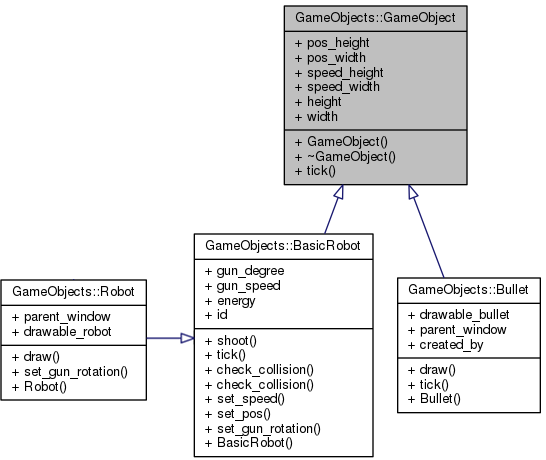
\includegraphics[scale = 0.7]{GameObjects_graph.png}
\caption{Game Objects UML Diagram}
\medskip
\end{figure}

\clearpage

\subsection{Game Server and Client}

\subsubsection{Server}
The gameserver consists of two different classes, first the actual game which calculates movements of objects, renders the them and finally sends an update via the server using grpc. The game server also prepares the data for the streaming server, which sends the all positions via asio to the player in order for them to see the whole game. The most important part of the gameserver is the ''game\_loop()'' function which covers all the functionalities that are described above.

\begin{figure}[h]
\centering
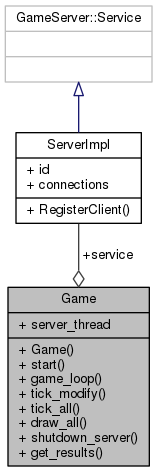
\includegraphics[scale = 0.7]{Game_graph.png}
\caption{Diagram of the game server}
\medskip
\end{figure}

\clearpage

\subsubsection{Client}
The client not only communicates with the server but also manages the players robot. The class prepares updates, sets the new position, speed etc. for the players convenience.

\begin{figure}[h]
\centering
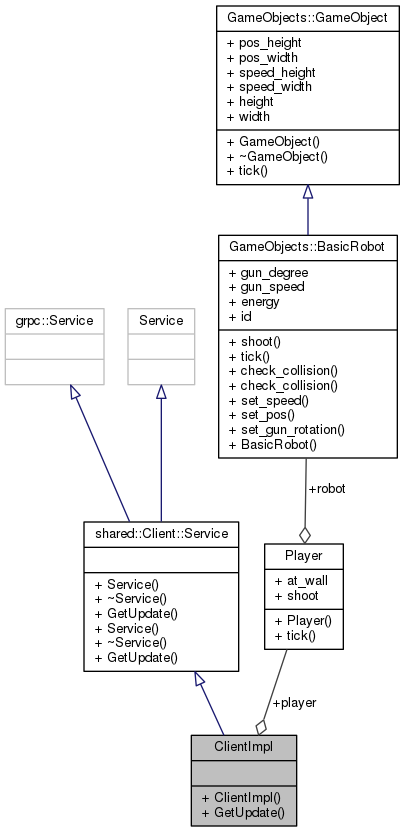
\includegraphics[scale = 0.5]{ClientImpl_graph.png}
\caption{Diagram of the client}
\medskip
\end{figure}

\subsection{Streaming server and client}
The streaming server and client are automatically started when hosting or connecting to a game. The streaming server continually sends an ''StreamingUpdate.proto'' message which the client can use to display the game state.

\begin{figure}[h]
\centering
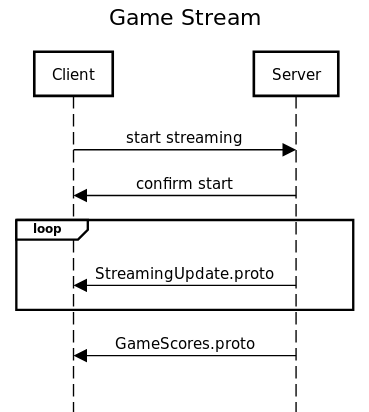
\includegraphics[scale = 0.5]{sequence_diagrm.png}
\caption{Diagram of the streaming sequence}
\medskip
\end{figure}

\section{Usage}

\subsection{Building the game}

The game can be build using either Meson or Cmake.

\subsubsection{Meson}
When building with Meson be sure to change all references in the ''meson.options'' files accordingly.

\subsubsection{Cmake}
For cmake to find all required library's the following environment variables have to be set:

\textbf{ASIO\_INCLUDE\_PATH} \\
Point to asio standalone include directory.

\textbf{SPDLOG\_INCLUDE\_PATH} \\
Point to spdlog/include directory.

\textbf{CLIPP\_INCLUDE\_PATH} \\
Point to clipp/include directory.

\textbf{JSON\_INCLUDE\_PATH} \\
Point to the directory where the ''json.hpp'' is located.

\subsection{Writing a robot}
For writing an own robot simply go to the file ''player.h'' and overwrite the example bot with your own one. The function ''tick()'' will be called every time the client receives an update from the server.

\lstset{language=C++,
                basicstyle=\ttfamily,
                keywordstyle=\color{blue}\ttfamily,
                stringstyle=\color{red}\ttfamily,
                commentstyle=\color{green}\ttfamily,
                morecomment=[l][\color{magenta}]{\#}
}
\scriptsize
\lstinputlisting[language=c++,style=protobuf]{code_listings/player.cpp}
\captionof{lstlisting}{Player.h}
\normalsize

Listing 3 is a simple wall bot example. The player robot circles around the walls while rotating his gun and shooting every time he scanned a robot. The program first searches for the lower wall and from there on travels clockwise near to the them.

\subsection{Hosting a game}
The game can be hosted by simply calling the built program via \lstinline{./robocode}. Then navigating the menu to ''Host a new game'' and ''Start getting connections'' using the arrow keys and the enter button. Then wait until at least two players have connected to the game and press enter on one of their names. \\

The game can also be hosted using the command \lstinline{./robocode -nmh}. ''-nhm'' stands for ''no-menu-host'' and means that the server will be started immediately and no menu will be displayed. \\

The ''-nhm'' option can also be set in the ''config.json'' file.

\subsection{Connecting to a game}
Again the player can simply use the menu to connect to a game. Call \lstinline{./robocode} again and navigate to ''Connect to a game''. Then type in an IP address in the ''Connect to'' field and press enter. The next window will open and requires a ''username'' to be typed in. \\

A connection can also be established using the command \lstinline{./robocode -c 127.0.0.1 username}. \\

Again this command can also be set in the configuration file by filling in the ''server\_ip'' and ''username'' parameter.

\end{document}

%This template was created by Roza Aceska.